\documentclass{amia}
\usepackage{graphicx}
\usepackage[labelfont=bf]{caption}
\usepackage[superscript,nomove]{cite}
\usepackage{color}
\usepackage{wrapfig}
\usepackage{hyperref}
\usepackage[normalem]{ulem}

\geometry{margin=1in,bottom=0mm}
\setlength{\voffset}{-.5in}

\begin{document}

\title{Creating RDF Data on Trauma Care Organizations from Questionnaires}

\author{Joseph R. Utecht, BA$^{1}$, Jonathan P. Bona, PhD$^{1}$, Mathias Brochhausen, PhD$^{1}$}

\institutes{
    $^1$University of Arkansas for Medical Science, Little Rock, AR, USA\\
}

\maketitle

\section*{Background}

Assessment of trauma systems and trauma centers positively affects patient outcomes \cite{ref1, ref2}.
However, assessment of these organizations often falls short because of a lack of comparability regarding components and their implementation.
The CAFE project (\href{https://cafe-trauma.com}{https://cafe-trauma.com}) aims to provide a web-based self-assessment environment for this domain.
To this end we develop a user-friendly questionnaire allowing respondents to enter data and compare organizational components in real time.
This poster describes our methodology to create semantically-rich data based on user-friendly, web-based questionnaires.


\section*{Methods}
To support our requirement of allowing user-friendly data entry, we developed a tool to create the appearance of a traditional web questionnaire.
To prevent any interruption for the respondent while the server processes previous answers, we chose to build the interface as a separate web application in Angular2 (\href{https://angular.io}{https://angular.io}).
To provide semantically-rich data, the server-side component will not only record the answer in a relational database, but simultaneously create a pre-configured RDF (\href{https://www.w3.org/RDF}{https://www.w3.org/RDF}) representation of the answer in a triplestore.

\section*{Results}
\begin{wrapfigure}{r}{0.35\textwidth}
  \vspace{-10mm}
  \begin{center}
    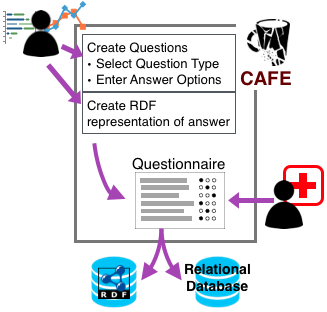
\includegraphics[width=0.33\textwidth]{pics/cafe_process6.png}
  \end{center}
  \caption{CAFE Process.}
  \label{cafe_process}
\end{wrapfigure}

The result of this work is available on Github (\href{https://github.com/cafe-trauma}{https://github.com/cafe-trauma}).
Fig. 1 shows the steps of acquiring RDF data through a questionnaire built using our tool.

The first step is the creation of the questions, for example ``Does your trauma center have a trauma registrar?". 
Next the administrative user defines the RDF representation for the answers, in this case, the representation of the trauma registrar, the trauma center, and the fact that the trauma registrar is an organizational member of that trauma center.
The tool then builds a traditional web questionnaire with a yes/no question ``Does your trauma center have a trauma registrar?"
As respondents answer this question the RDF representation is created in a triplestore and their answer is recorded in a relational database.

From the respondent's point of view the questionnaire does not differ in any way from a typical web questionnaire.
The benefit of this method is that the data about a respondent's organization is available in a format that allows integration with rich semantic resources.
In the CAFE project we use the OWL ontology OOSTT \cite{ref3} to integrate knowledge about trauma systems and trauma centers.

\section*{Discussion}
The methodology presented in this paper is not restricted to the domain of the CAFE project, but is applicable to multiple domains of biomedical research and medicine.
In addition to trauma care, we have also successfully implemented questionnaires collecting data on potential drug-drug interactions using this methodology.

\section*{Acknowledgements}
The research presented in this paper is funded by the National Institute of General Medical Sciences of the National Institutes of Health under award number \textbf{1R01GM111324}.

\makeatletter
\renewcommand{\@biblabel}[1]{\hfill #1.}
\makeatother

\bibliographystyle{unsrt}
\begin{thebibliography}{1}
\setlength\itemsep{-0.1em}

\bibitem{ref1}
T.L.Sanddal, T.J.Esposito, J.R.Whitney, D.Hartford, P.P.Taillac, N. C. Mann NC, et al.. ``Analysis of preventable trauma deaths and opportunities for trauma care improvement in Utah," J Trauma. 2011 Apr;70(4):970-7.

\bibitem{ref2}
T. J. Esposito, T. L. Sanddal, S. A. Reynolds, N. D. Sanddal, ``Effect of a voluntary trauma system on preventable death and inappropriate care in a rural state," J Trauma, 2003, 54(4), 663-670.

\bibitem{ref3}
Utecht J, Judkins J, Colvin T Jr., et al. OOSTT: a Resource for Analyzing the Organizational Structures of Trauma Centers and Trauma Systems. CEUR Workshop Proc. 2016 Aug;1747. \href{http://ceur-ws.org/Vol-1747/IT504_ICBO2016.pdf}{http://ceur-ws.org/Vol-1747/IT504\_ICBO2016.pdf}

\end{thebibliography}

\end{document}
